Der Aufbau der Messapparatur ist schematisch in Abbildung \ref{fig:aufbau} dargestellt.
\begin{figure}[h!]
  \centering
  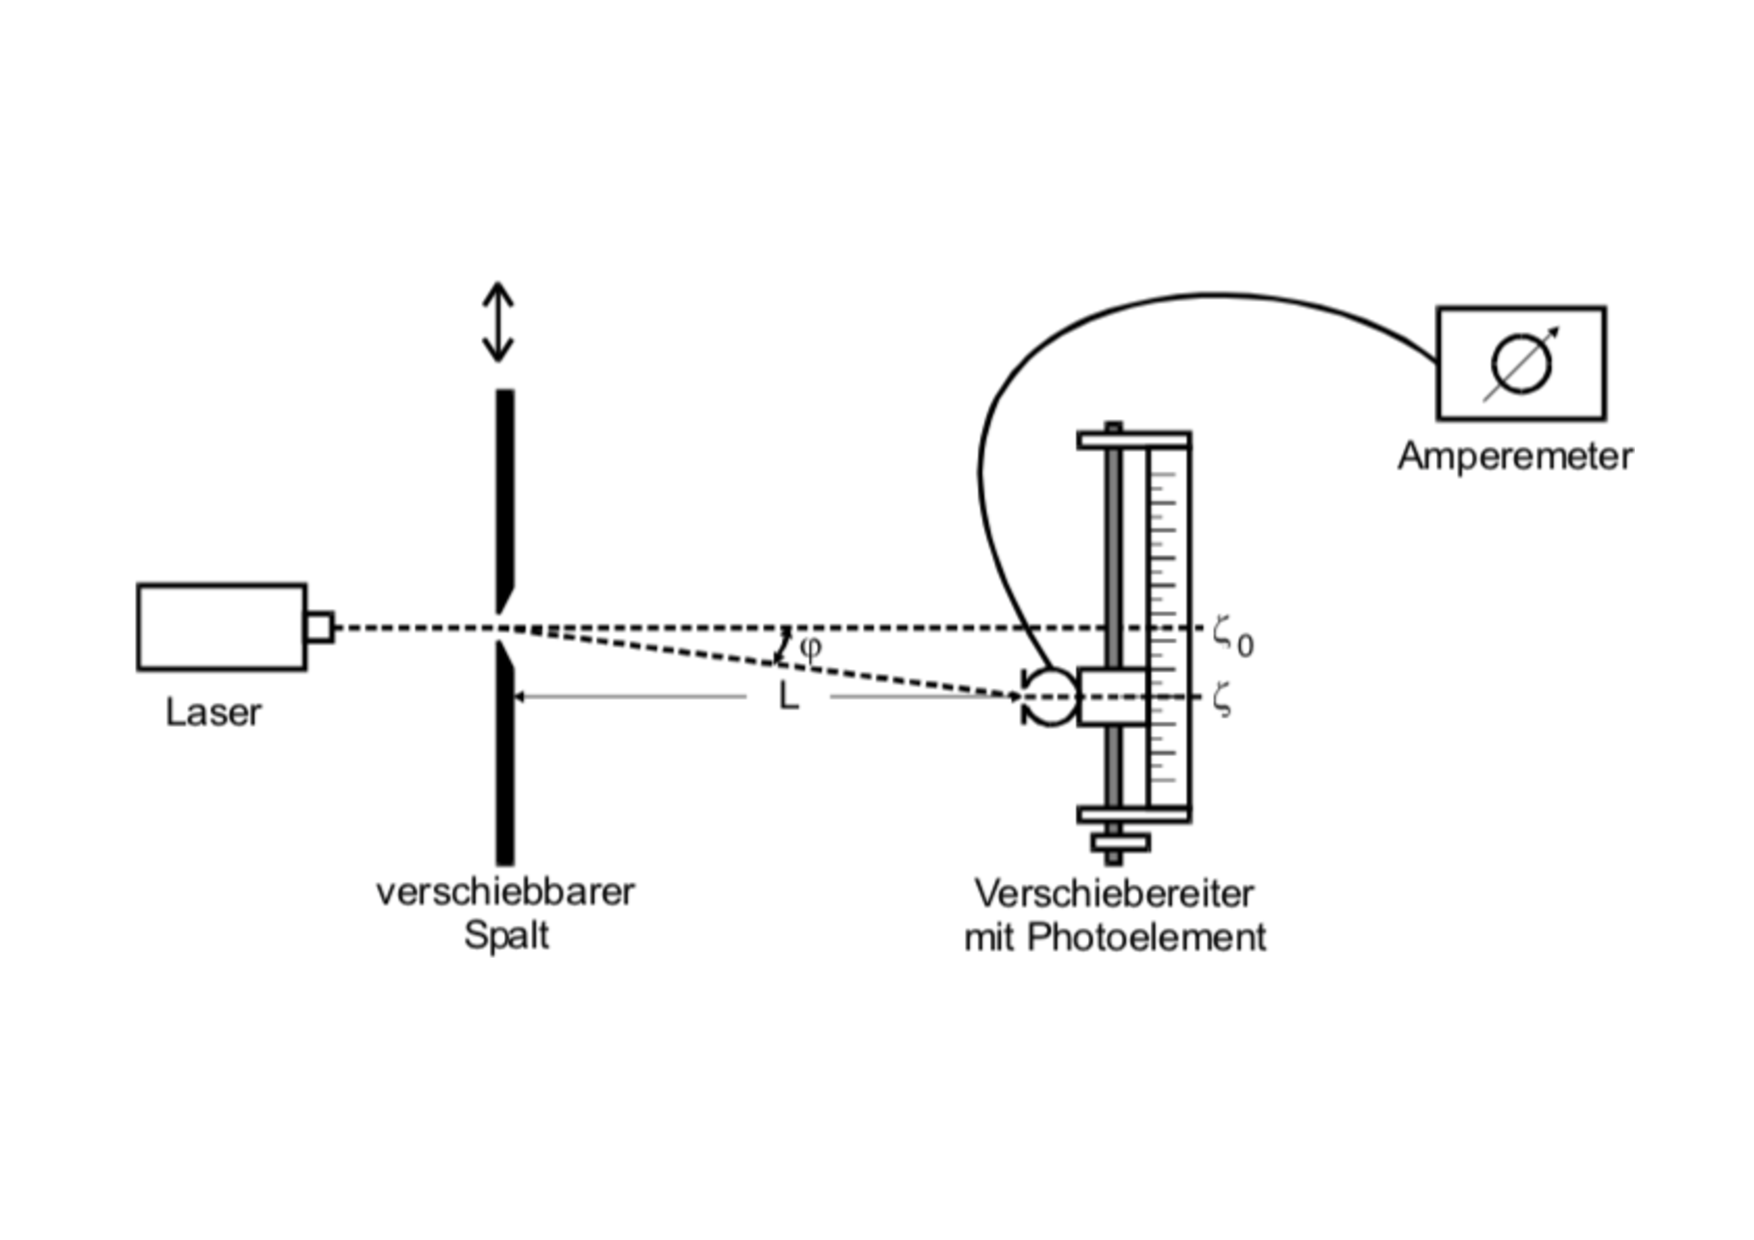
\includegraphics[width=\textwidth]{aufbau.pdf}
  \caption{Aufbau der Messapparatur \cite{1}}
  \label{fig:aufbau}
\end{figure}
Ein Laser der Wellenlänge $\lambda=\SI{00000000000000}{}$ ist mit einer Blende zum Befestigen der Spalte und einem Detektor auf einer Schiene angebracht.
Der Spalt und der Detektor liegen in einem Abstand von $L=\SI{0.9}{m}$.
Die Lichtwellen des Lasers fallen auf einen der Spalte, werden gebeugt und an dem seitlich verschiebbaren Detektor zeigt sich ein jeweiliges Interferenzmuster.
Der Detektor bildet die einfallende Intensität als Strom ab.
Der Strom wird mit einem Amperemeter gemessen.
\\Initial wird der 'Dunkelstrom' $I_{\text{du}}=\SI{0.58}{nA}$ gemessen.
Er zeigt an, wie groß das Untergrundrauschen durch die sonstigen Lichtquellen und ohne den Laser ist.
\\Zunächst wird ein Einzelspalt der Breite $b=\SI{0.022e-3}{m}$ untersucht.
Das Interferenzmuster wird per Hand möglichst genau auf den Detektor gerichtet.
Dann wird das Intensitätsmaximum lokalisiert und der Detektor wird  bei der Messung seitlich verschoben, um die Intensität in Abhängigkeit zum Ort zu messen.
Dann wird der Strom in $\Delta \zeta =\SI{0.5}{mm}$-Schritten gemessen.
Bei den Intensitätsminima und -maxima werden weitere Messwerte aufgenommen.
Es werden das Hauptmaximum und die nächsten zwei Nebenmaxima in beide Richtungen untersucht.
\\Der zweite untersuchte Einzelspalt hat die Weite $b= \SI{0.1e-3}{m}$.
Die Messung erfolgt analog zu der vorherigen Messung.
\\Zuletzt wird ein Doppelspalt untersucht.
Die Spaltweite beträgt $b= \SI{0.15e-3}{m}$ und der Spaltabstand beträgt $g=\SI{0.25e-3}{m}$.
Das Intensitätsmaximum wird ermittelt und die Intensität wird in Abhängigkeit des Abstands zum Intensitätsmaximum gemessen.


\FloatBarrier
